\documentclass[preprint2]{aastex}

%% preprint2 produces a double-column, single-spaced document:

%% \documentclass[preprint2]{aastex}

%% Sometimes a paper's abstract is too long to fit on the
%% title page in preprint2 mode. When that is the case,
%% use the longabstract style option.

%% \documentclass[preprint2,longabstract]{aastex}

%% If you want to create your own macros, you can do so
%% using \newcommand. Your macros should appear before
%% the \begin{document} command.
%%
%% If you are submitting to a journal that translates manuscripts
%% into SGML, you need to follow certain guidelines when preparing
%% your macros. See the AASTeX v5.x Author Guide
%% for information.

\usepackage{graphicx}
%\usepackage{caption}
%\usepackage{subcaption}
\usepackage{subfigure}

\newcommand{\vdag}{(v)^\dagger}
\newcommand{\myemail}{}
\newcommand{\pflux}{photons cm$^{-2}$ s$^{-1}$}
\newcommand{\lsi}{LS~I~+61~303}

%% You can insert a short comment on the title page using the command below.


%% If you wish, you may supply running head information, although
%% this information may be modified by the editorial offices.
%% The left head contains a list of authors,
%% usually a maximum of three (otherwise use et al.).  The right
%% head is a modified title of up to roughly 44 characters.
%% Running heads will not print in the manuscript style.

\shorttitle{Exceptionally Bright TeV Emission From the Binary LS I +61 303}
\shortauthors{}

%% This is the end of the preamble.  Indicate the beginning of the
%% paper itself with \begin{document}.

\begin{document}

%% LaTeX will automatically break titles if they run longer than
%% one line. However, you may use \\ to force a line break if
%% you desire.

\title{Exceptionally Bright TeV Emission From the Binary \lsi{}}

%% Use \author, \affil, and the \and command to format
%% author and affiliation information.
%% Note that \email has replaced the old \authoremail command
%% from AASTeX v4.0. You can use \email to mark an email address
%% anywhere in the paper, not just in the front matter.
%% As in the title, use \\ to force line breaks.

\author{
Andy Smith\altaffilmark{1},
Anna OFdB\altaffilmark{2},
VERITAS Collaboration\altaffilmark{3}
}

%% Notice that each of these authors has alternate affiliations, which
%% are identified by the \altaffilmark after each name.  Specify alternate
%% affiliation information with \altaffiltext, with one command per each
%% affiliation.

\altaffiltext{1}{America}
\altaffiltext{2}{Germany}
\altaffiltext{3}{Everywhere}

%% Mark off your abstract in the ``abstract'' environment. In the manuscript
%% style, abstract will output a Received/Accepted line after the
%% title and affiliation information. No date will appear since the author
%% does not have this information. The dates will be filled in by the
%% editorial office after submission.

\begin{abstract}
The TeV binary system \lsi{} is known for its regular, although not entirely understood, non-thermal emission pattern, which traces the orbital period of the compact object in its 26.5 day orbit around its Be star companion. When active in the TeV regime, the system typically presents elevated emission around apastron passage with flux levels in the 5-15$\%$ Crab Nebula range (above 350 GeV). Here we present VERITAS observations of \lsi{} taken in late 2014, which detected large TeV flares around apastron at flux levels peaking above 30$\%$ of the Crab Nebula flux, the brightest such activity ever seen in the TeV regime. We also provide a confirmation of the off-apastron emission previously seen by VERITAS. The strong outbursts observed have rise times of 1-2 days and a typical 1-2 day duration; during the 2014 observations \lsi{} was seen to go from a quiescent TeV state to one in which $>$10 TeV emission was detected from the system. This short acceleration time for particles (for galactic scale objects) provides strong constraints on the nature of the accelerating mechanism in \lsi{}.


\end{abstract}


\keywords{}

\section{Introduction}

The current generation of Imaging Atmospheric Cherenkov Telescopes (IACTs) has opened up the study of the class of high hass X-ray binary star systems which also present TeV emission on various timescales. The class of these TeV binaries is quite sparse, consisting of only a handful of sources: LS 5039, PSR B1259-63, \lsi{}, HESS J0632+057 and HESS J1018-589. Of these, only the compact object of PSR B1259-63 has been firmly identified as a pulsar; the rest of the TeV binaries still have a large degree of ambiguity about the nature of the compact object within the system and, consequently, the fundamental setup which produces the TeV emission along with its characteristic variability. For instance, the presence of a pulsar within a given TeV binary indicates that the emission in the system is generated by the shock formed at the interface between the pulsar and stellar winds. The variability would therefore be driven principally by the varying density of the stellar wind density that the pulsar ``sees'' in its orbit. In the case of a black hole companion, the emission would be driven by an accretion driven jet. Modeling of the emission from these objects has driven a very active field with models falling into both of the above categories (binary pulsar vs micro quasar), as well as utilizing both leptionic and hadronic emission models. As more ``direct'' attempts to measure the nature of the systems in question have yet to yield decisive information (for example, constraining the inclination angle of viewing to narrow the compact mass down to rule out a black hole) the way forward appears to be provide further monitoring of the systems across the spectrum in the hopes of discovering some observational feature that would firmly identify these systems and the basic interacting parts within them. The TeV emission in these sources is correlated with the orbital periods of their compact objects; since the orbital periods vary from several days (LS 5039) to several years (PSR B129-63), the various sources can sometimes only present a short duty cycle for study in the TeV regime. Of the TeV binaries, \lsi{} is the only source in the Northern Hemisphere which has a short enough orbital period (26.5 days) to allow for regular study with TeV instruments. This has made it an excellent target for Northern Hemisphere TeV observatories. 

\lsi{} is a high mass X-ray binary system at a distance of $\sim2$ kpc, composed of a B0 Ve star and a compact object. The observed radio through optical emission is modulated with a period of $P \approx 26.5$ days, believed to be associated with the orbital period of the binary system [refs]. Radial velocity measurements show the orbit to be elliptical ($e = 0.537\pm0.034$), with periastron passage occurring around phase $\phi=0.275$, apastron passage at $\phi=0.775$, superior conjunction at $\phi=0.081$ and inferior conjunction at $\phi=0.313$ (Aragona et al. 2009).

As a TeV source, \lsi{} has presented puzzling behavior. Initial detections in 2006\,--\,2007 by both the VERITAS and MAGIC collaborations [refs] over many orbital cycles showed the source to be a variably bright TeV source, with emission peaking around apastron passage (see Figure 1). Subsequent observations in 2008\,--\,2010 [12] showed no evidence for emission during these previously detected phases, instead only detecting the source at a lower TeV flux near the periastron passage of a single orbit. 

However, VERITAS observations taken in Nov-Dec 2011 showed the source to be highly active around apastron again [refs], similar to the behavior observed in 2006\,--\,2007. In both the 2011\,--\,2012, and 2012\,--\,2013 timeframes, both MAGIC and VERITAS saw the source at only typical emission levels [refs], i.e., $5-15\%$ of the Crab Nebula above 300 GeV. In this work we present the results of the VERITAS campaign on \lsi{} during the Fall of 2014. During this time, VERITAS observed \lsi{} to be flaring at historically high flux levels with the source presented flux levels a factor of 2-3 higher than seen previously. 


\section{Observations}
The VERITAS IACT array, located at the base of Mt. Hopkins, AZ (1.3 km a.s.l., 31$^{\circ}$40'30"N, 110$^{\circ}$57'07" W) consists of four Davies-Cotton design optical telescopes (12m diameter). Each VERITAS telescope consists of 350 hexagonal mirror facets which focus Cherenkov flashes created by gamma-ray air showers in the atmosphere onto a pixelated photo-multiplier tube (PMT) camera consisting of 499 Hamamatsu Blah Blah high QE PMTs. VERITAS is sensitive in the energy range of 85 GeV to 30 TeV and has the ability to detect a 1$\%$ Crab Nebula source in approximately 25 hours. For a full description of the hardware components and analysis methods utilized by VERITAS, please see [][].

In the 2014 season, VERITAS observations of \lsi{} were taken from October 16 (MJD 56946) to  December 12 (MJD 57003), obtaining a total of 24.7 hours of quality selected livetime observations. These observations covered three separate orbits of \lsi{}, sampling the orbital regions of $\phi = 0.5-0.2$ (see Figure~\ref{f:fig1}). For the entire observation set, a total of 449 excess events above background were detected, equivalent to significance of 21$\sigma$.

\begin{figure}[ht]
\centering
\subfigure[\label{fig1}]{
  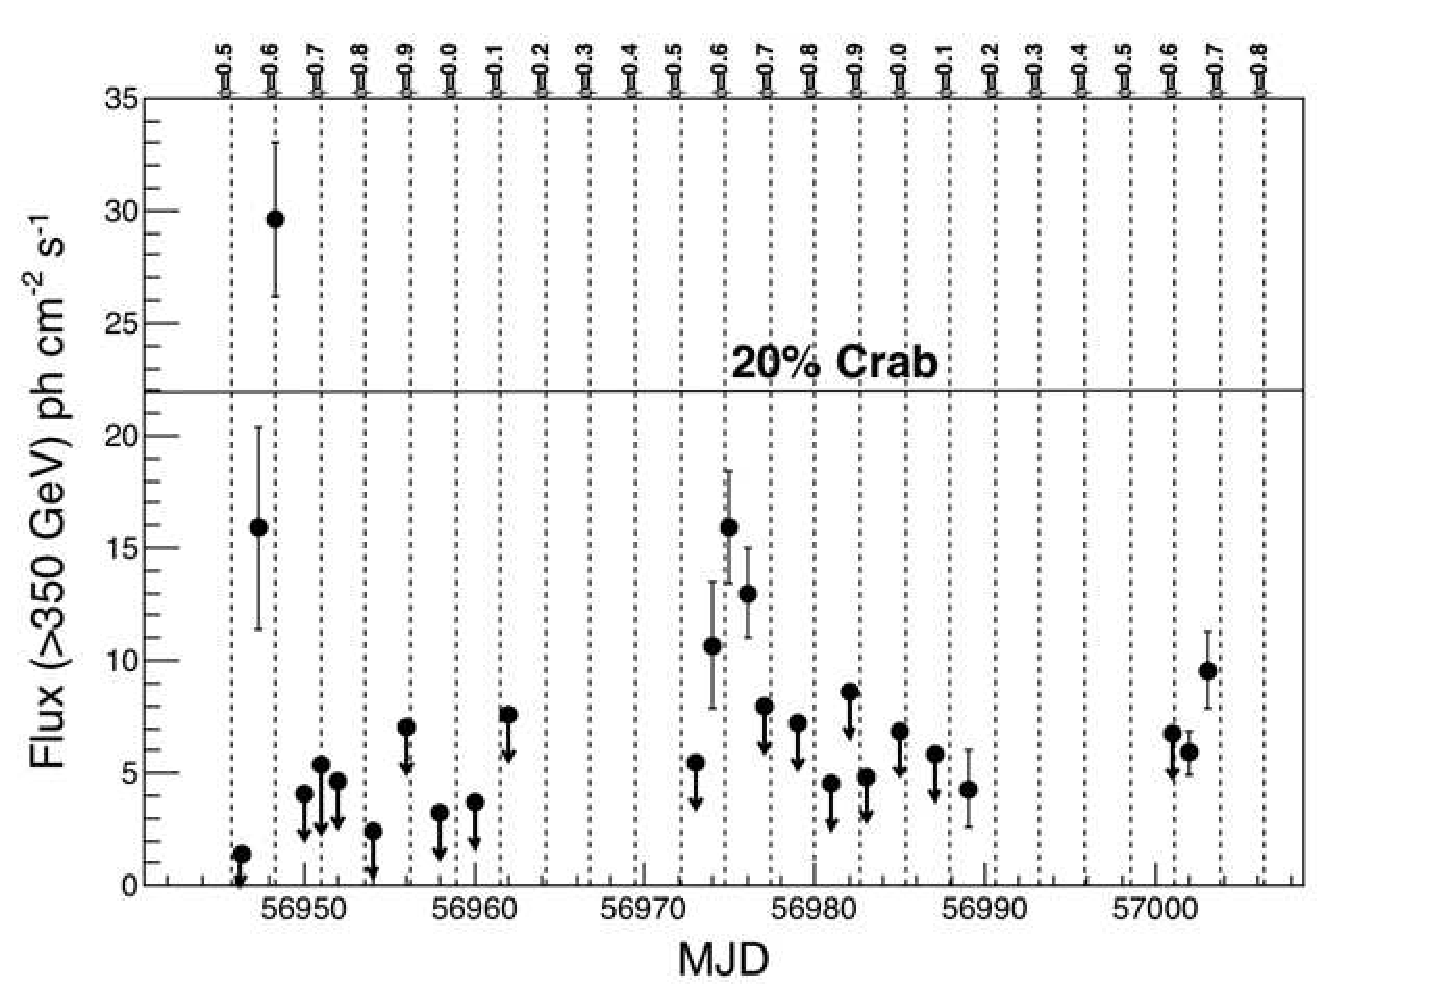
\includegraphics[width=0.5\textwidth]{./Figure1.pdf}
  %\caption{The VERITAS $>$350 GeV light curve of \lsi{} during the 2014 observation season (\textbf{VEGAS}).} 
  %\label{fig1}
}
\subfigure[\label{fig1b}]{
  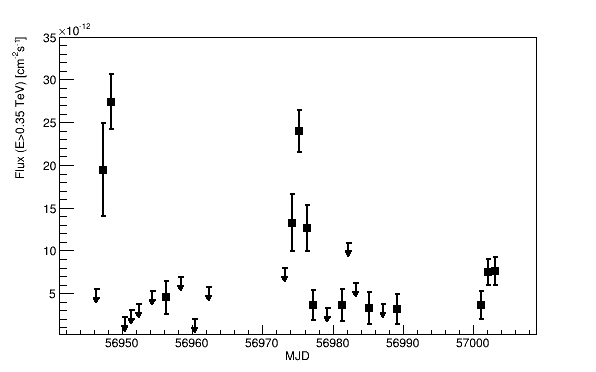
\includegraphics[width=0.5\textwidth]{figs/LSI-mod-lc-days-gt350gev.png}
  %\caption{The VERITAS $>$350 GeV light curve of \lsi{} during the 2014 observation season (\textbf{ED}).}
  %\label{fig1b}
}
\caption{The VERITAS $>$350 GeV light curve of \lsi{} during the 2014 observation season from \textbf{VEGAS}~\subref{fig1} and \textbf{ED}~\subref{fig1b}.}
\label{f:fig1}
\end{figure}

During the first orbit observed (in October), the source presented the largest of its flares (hereafter "F1"), beginning on 17 October 2014 (MJD 56947, $\phi =  0.55$) with emission reaching a peak of $3.0 \pm 0.3 \times10^{-11}$ \pflux{} ($>$350 GeV) on October 18 (MJD 56948). This flare peaked at approximately $30\%$ of the Crab Nebula flux in the same energy range and represents the largest flux ever detected from the source. Unfortunately, poor weather conditions limited observations for the next few nights after this peak and only recommenced on October 20 (MJD 56950), when the source had already quietened down. As can be seen in Figure 1, this flare is rather sharply defined: only one night before the flare began, the source was in a quescient state with a $99\%$ confidence upper limit of emission of $1.4 \times10^{-11}$ \pflux{} ($>$350 GeV). This fast rising behavior confirms the result of [ref].

During the November observation (second orbital passage), VERITAS detected another period of high activity for the source at similar orbital phases ($\phi = 0.5-0.6$) with similar flux levels detected. Additionally, during this orbit, VERITAS detected emission from the source during off-apastron passage phases of 0.1. This result confirms the initial detection of off-apastron emission presented in []. Follow-up observations conducted by VERITAS during the next month (December 10-12, 2014) covered the orbital phases of $\phi=0.59-0.67$ and detected the source at a lower flux level of $\sim1.7\times10^{-11}$ \pflux{} ($>$350 GeV).

During the 2014 observing season, the differential energy spectrum of \lsi{} was consistent with past observations, i.e., the emission in the 0.2-25 TeV is well fit by a power-law described by $\left( 1.92 \pm 0.12_{\mathrm{stat}} \times 10^{-8} \right) \times \left( \frac{E}{\mathrm{1 TeV}} \right)^{-2.56 \pm 0.08_{\mathrm{stat}}}$ TeV$^{-1}$ m$^{-2}$ s$^{-1}$, see Figure~\ref{spec}.

\begin{figure}
\centering
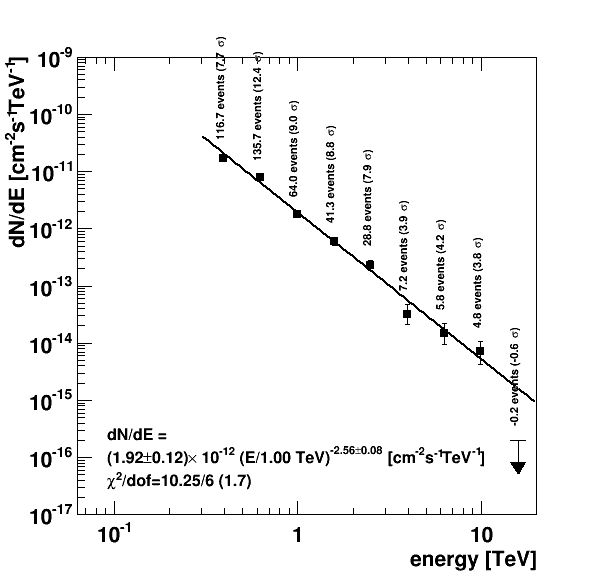
\includegraphics[width=0.5\textwidth]{figs/LSI-mod-replot-spec.png}
\caption{Average differential energy spectrum of \lsi{}.}
\label{spec}
\end{figure}

During these observations, the source was also being monitored by \emph{Fermi}-LAT ($0.1\,--\,300$ GeV), \emph{Swift}-XRT ($0.2\,--\,10$ keV), and both the RATAN and AMI radio instruments (Ghz??). In addition, H-alpha monitoring of the system was taking place with the Ritter Observatory in Toledo, Ohio (USA). After the second flare (November) was detected by VERITAS, Atel $\#$6785 was released, notifying the astronomical community of the historic flux levels which triggered more intense observations with the existing multiwavelength partners, as well as additional observations with the MAGIC TeV observatory in the Canary Islands [refs]. The results of this campaign are under analysis and will be presented in an upcoming publication. 


\section{Discussion and Interpretation}





\end{document}

%%
%% End of file `sample.tex'.
